\documentclass[11pt,a4paper]{article}
\usepackage[margin=2cm]{geometry}
\usepackage[T1]{fontenc}
\usepackage[utf8]{inputenc}
\usepackage{hyperref}
\usepackage{xcolor}
\usepackage{listings}
\usepackage{tikz}
\usetikzlibrary{positioning,arrows.meta}
\definecolor{codebg}{RGB}{248,250,252}
\definecolor{codeblue}{RGB}{37,99,235}
\definecolor{codegreen}{RGB}{22,101,52}
\definecolor{codered}{RGB}{185,28,28}
\definecolor{codegray}{RGB}{100,116,139}
\lstdefinelanguage{JavaScript}{morekeywords={const,let,var,async,await,function,try,catch,return,if,else,for,of,require,module,exports},sensitive=true,morecomment=[l]{//},morestring=[b]",morestring=[b]`}
\lstdefinestyle{prokuraCode}{basicstyle=\ttfamily\small,breaklines=true,frame=single,columns=fullflexible,keepspaces=true,showspaces=false,showstringspaces=false,showtabs=false,tabsize=2,numbers=left,numberstyle=\tiny\color{codegray},keywordstyle=\color{codeblue}\bfseries,stringstyle=\color{codered},commentstyle=\color{codegreen},rulecolor=\color{codegray},backgroundcolor=\color{codebg}}
\lstset{style=prokuraCode}
\newcommand{\docheader}[2]{
\begin{titlepage}
\centering
{\Large\bfseries Prokura HoReCa Supply\par}
\vspace{0.4cm}
{\large Dokumentasi Fitur Microservice Final Project\par}
\vspace{0.8cm}
{\large Mata Kuliah: Proyek 2 - Final Project\par}
\vspace{1.2cm}
{\large\bfseries #1\par}
{\large NIM: #2\par}
\vfill
\begin{tabular}{rl}
Program Studi: & Ilmu Komputer\\
Departemen: & Departemen Ilmu Komputer dan Elektronika (DIKE)\\
Fakultas: & FMIPA\\
Universitas: & Universitas Gadjah Mada\\
\end{tabular}
\vfill
\end{titlepage}
}

\begin{document}
\docheader{Ravif Gayuh Wicaksono}{24/540583/PA/22953}

\section*{Peran}
Owner Catalog Service. Ravif bertanggung jawab pada data produk, penambahan SKU baru, katalog, pencarian, dan filter produk.

\section*{Bukti Microservice}
Catalog Service sudah dipisahkan sebagai service boundary di \path{prokura-api/src/services/catalog}. API gateway di \path{prokura-api/server.js} memasang route Catalog, sedangkan \path{prokura-api/src/service-host.js} dapat menjalankan service tunggal bernama \texttt{catalog}.

Lokasi kode: \path{prokura-api/src/service-host.js}

\begin{lstlisting}[language=JavaScript]
const serviceRegistry = {
  catalog: registerCatalogRoutes,
  customer: registerCustomerRoutes,
  inventory: registerInventoryRoutes,
  order: registerOrderRoutes,
  reporting: registerReportingRoutes,
};
\end{lstlisting}

Penjelasan: registry ini membuktikan tiap domain punya route module sendiri. Saat \texttt{SERVICE\_NAME=catalog} atau command \texttt{node src/service-host.js catalog} dijalankan, host hanya memasang route Catalog Service. Ini sesuai keinginan dosen karena integrasi sistem dilakukan lewat endpoint API, bukan query database langsung dari UI.

\section*{Tanggung Jawab Fitur}
\begin{enumerate}
\item Penambahan barang baru.
\item Pencarian dan filter barang.
\end{enumerate}

\section*{Diagram Tabel yang Ditangani}
\begin{center}
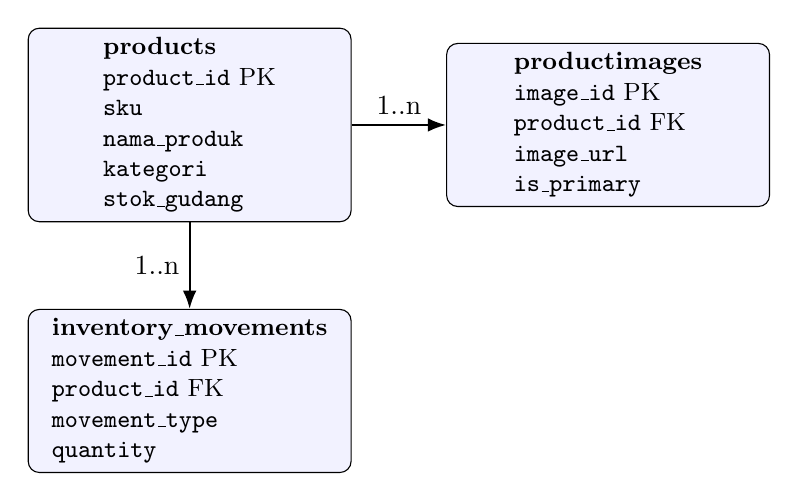
\begin{tikzpicture}[entity/.style={draw, rounded corners, fill=blue!5, align=left, font=\small, minimum width=4.1cm}, rel/.style={-Latex, thick}]
\node[entity] (products) {\textbf{products}\\\texttt{product\_id} PK\\\texttt{sku}\\\texttt{nama\_produk}\\\texttt{kategori}\\\texttt{stok\_gudang}};
\node[entity, right=1.2cm of products] (images) {\textbf{productimages}\\\texttt{image\_id} PK\\\texttt{product\_id} FK\\\texttt{image\_url}\\\texttt{is\_primary}};
\node[entity, below=1.1cm of products] (movements) {\textbf{inventory\_movements}\\\texttt{movement\_id} PK\\\texttt{product\_id} FK\\\texttt{movement\_type}\\\texttt{quantity}};
\draw[rel] (products) -- node[above]{1..n} (images);
\draw[rel] (products) -- node[left]{1..n} (movements);
\end{tikzpicture}
\end{center}

Penjelasan: Catalog Service terutama mengelola tabel \texttt{products}. Tabel \texttt{productimages} dipakai saat katalog menampilkan gambar utama, sedangkan \texttt{inventory\_movements} tersentuh saat produk baru dibuat dengan stok awal.

\section*{Lokasi Kode Program dan Penjelasan}
\subsection*{Route tambah dan cari produk}
Lokasi kode: \path{prokura-api/src/services/catalog/routes.js}

\begin{itemize}
\item \texttt{GET /api/products}: line 11.
\item \texttt{POST /api/products}: line 21.
\end{itemize}

\begin{lstlisting}[language=JavaScript]
app.get("/api/products", async (req, res) => {
  try {
    const filters = buildProductSearchFilters(req.query);
    const products = await listProducts(pool, filters);
    res.json({ success: true, data: products });
  } catch (error) {
    sendError(res, error, "Gagal mengambil katalog produk");
  }
});
\end{lstlisting}

Penjelasan: endpoint ini menerima query string dari UI, menormalisasi filter melalui domain helper, lalu memanggil repository \texttt{listProducts}. Hasilnya dikembalikan sebagai JSON agar admin dan customer web dapat menampilkan katalog tanpa akses database langsung.

\begin{lstlisting}[language=JavaScript]
app.post("/api/products", async (req, res) => {
  const client = await pool.connect();
  try {
    const { sku, nama_produk, kategori, satuan, harga_dasar, stok_gudang } = req.body;
    if (!nama_produk || !satuan || !harga_dasar) {
      return res.status(400).json({ success: false, message: "Data produk tidak lengkap" });
    }

    let normalizedSku;
    try {
      normalizedSku = normalizeSku(sku);
    } catch (error) {
      return res.status(400).json({ success: false, message: error.message });
    }
\end{lstlisting}

Penjelasan: endpoint tambah produk memvalidasi data wajib dan menormalisasi SKU sebelum insert. Validasi ini mencegah data katalog tidak lengkap masuk ke database.

\begin{lstlisting}[language=JavaScript]
    await client.query("BEGIN");
    const product = await createProduct(client, {
      sku: normalizedSku,
      nama_produk,
      kategori,
      satuan,
      harga_dasar,
      stok_gudang,
    });

    if (Number(stok_gudang || 0) > 0) {
      await recordInventoryMovement(client, {
        productId: product.product_id,
        movementType: "INITIAL_STOCK",
        quantity: Number(stok_gudang || 0),
        note: "Stok awal saat produk dibuat",
        referenceType: "PRODUCT",
        referenceId: product.product_id,
      });
    }

    await client.query("COMMIT");
    res.status(201).json({ success: true, data: product });
\end{lstlisting}

Penjelasan: insert produk dan pencatatan stok awal berjalan dalam transaksi yang sama. Kalau produk baru punya stok awal, Catalog Service memanggil pencatatan movement \texttt{INITIAL\_STOCK} sehingga Inventory Service tetap punya audit trail.

\subsection*{SQL repository katalog}
Lokasi kode: \path{prokura-api/src/services/catalog/repository.js}

\begin{itemize}
\item Query list/search produk: line 22.
\item Insert produk baru: line 37.
\end{itemize}

\begin{lstlisting}[language=JavaScript]
if (filters.q) {
  params.push(`%${filters.q}%`);
  conditions.push(`(p.nama_produk ILIKE $${params.length} OR p.sku ILIKE $${params.length})`);
}

if (filters.category) {
  params.push(filters.category);
  conditions.push(`p.kategori = $${params.length}`);
}
\end{lstlisting}

Penjelasan: bagian ini membangun filter pencarian berdasarkan nama/SKU dan kategori dengan parameter query PostgreSQL. Parameter dipisahkan dari string SQL untuk mengurangi risiko SQL injection.

\begin{lstlisting}[language=JavaScript]
const { rows } = await pool.query(
  `
    SELECT p.product_id, p.sku, p.nama_produk, p.kategori, p.satuan,
           p.harga_dasar, p.stok_gudang, i.image_url
    FROM products p
    LEFT JOIN productimages i ON p.product_id = i.product_id AND i.is_primary = TRUE
    ${where}
    ORDER BY p.nama_produk ASC
  `,
  params,
);
\end{lstlisting}

Penjelasan: query ini mengambil produk beserta gambar utama jika ada, menerapkan filter yang sudah dibuat, lalu mengurutkan produk berdasarkan nama.

\begin{lstlisting}[language=JavaScript]
const { rows } = await client.query(
  `
    INSERT INTO products (sku, nama_produk, kategori, satuan, harga_dasar, stok_gudang)
    VALUES ($1, $2, $3, $4, $5, $6)
    RETURNING product_id, sku, nama_produk, kategori, satuan, harga_dasar, stok_gudang
  `,
  [
    product.sku,
    product.nama_produk,
    product.kategori || null,
    product.satuan,
    product.harga_dasar,
    product.stok_gudang || 0,
  ],
);
\end{lstlisting}

Penjelasan: query insert ini membuat produk baru dan langsung mengembalikan data produk yang baru dibuat. Return value dipakai API untuk menampilkan feedback sukses ke UI.

\subsection*{UI admin dan customer}
Lokasi kode: \path{prokura-admin/app3.py}, menu \texttt{Manajemen Stok Gudang}, line 399 dan form \texttt{Tambah Produk Baru} line 463. Lokasi customer web: \path{prokura-web/app/page.tsx}, fetch produk line 58 dan search input line 264.

\begin{lstlisting}[language=JavaScript]
fetch(`${API_BASE_URL}/api/products`).then((r) => r.json()),
\end{lstlisting}

Penjelasan: customer web mengambil katalog melalui API gateway, bukan database langsung.

\begin{lstlisting}[language=JavaScript]
<input
  value={searchTerm}
  onChange={(event) => setSearchTerm(event.target.value)}
  placeholder="Cari produk atau SKU..."
\end{lstlisting}

Penjelasan: input ini menjadi kontrol pencarian di customer web. Nilai \texttt{searchTerm} dipakai untuk memfilter produk berdasarkan nama atau SKU di sisi UI setelah data katalog diterima dari API.

\section*{SQL Query Demo dan Penjelasan}
\subsection*{Query 1: tambah produk}
\begin{lstlisting}[language=SQL]
INSERT INTO products (sku, nama_produk, kategori, satuan, harga_dasar, stok_gudang)
VALUES ('SKU-DEMO-001', 'Demo Product', 'Bahan Pokok', 'Kg', 25000, 50)
RETURNING product_id, sku, nama_produk, kategori, satuan, harga_dasar, stok_gudang;
\end{lstlisting}

Penjelasan: query ini menambahkan satu produk baru ke tabel \texttt{products}. Bagian \texttt{RETURNING} dipakai untuk membuktikan row benar-benar masuk dan untuk melihat \texttt{product\_id} yang dibuat PostgreSQL.

\subsection*{Query 2: cari produk}
\begin{lstlisting}[language=SQL]
SELECT p.product_id, p.sku, p.nama_produk, p.kategori, p.satuan,
       p.harga_dasar, p.stok_gudang
FROM products p
WHERE p.nama_produk ILIKE '%demo%'
   OR p.sku ILIKE '%demo%'
ORDER BY p.nama_produk ASC;
\end{lstlisting}

Penjelasan: query ini mencari produk dengan keyword \texttt{demo} pada nama produk atau SKU. \texttt{ILIKE} membuat pencarian tidak sensitif huruf besar/kecil. Hasilnya menunjukkan produk yang baru ditambahkan bisa ditemukan dari katalog.

\section*{Alur Demo}
\subsection*{A. Penambahan barang baru}
\begin{enumerate}
\item Jalankan SQL \texttt{SELECT} berdasarkan SKU demo untuk menunjukkan produk belum ada atau mencatat kondisi awal.
\item Buka admin \texttt{Manajemen Stok Gudang}.
\item Masuk ke tab \texttt{Tambah Produk Baru}.
\item Isi SKU, nama produk, kategori, satuan, harga dasar, dan stok awal.
\item Submit form.
\item Tunjukkan response sukses dan data produk baru.
\item Jalankan SQL \texttt{SELECT} ulang untuk menunjukkan row baru di \texttt{products}.
\end{enumerate}

\subsection*{B. Pencarian dan filter barang}
\begin{enumerate}
\item Buka katalog produk di admin atau customer web.
\item Ketik nama/SKU produk demo pada search input.
\item Pilih kategori jika ingin menunjukkan filter kategori.
\item Tunjukkan hanya produk yang cocok yang tampil.
\item Hubungkan tampilan UI dengan endpoint \texttt{GET /api/products} dan query \texttt{ILIKE} pada repository.
\end{enumerate}

\section*{Bukti Validasi}
\begin{itemize}
\item Unit test Catalog: \path{prokura-api/tests/unit/catalog-domain.test.js}.
\item Repository test Catalog: \path{prokura-api/tests/unit/repository.test.js}.
\item Integration test lintas service: \path{prokura-api/tests/integration/api-final-project.test.js}.
\item Smoke test final project membuat produk dan mencari produk baru.
\end{itemize}

\end{document}
